\documentclass[border=6pt,tikz]{standalone}
\usepackage{tikz}
\usepackage{amsmath,amssymb}
\usetikzlibrary{arrows.meta,positioning,fit,backgrounds,calc,shapes.geometric,decorations.pathreplacing,patterns}
\definecolor{ink}{HTML}{1B2430}
\definecolor{muted}{HTML}{6B7785}
\definecolor{accent}{HTML}{2F6FB5}
\definecolor{accent2}{HTML}{C1611F}
\definecolor{good}{HTML}{2E7D5B}
\definecolor{soft}{HTML}{EDF2F7}
\definecolor{soft2}{HTML}{FBEDE2}
\definecolor{soft3}{HTML}{E6F0E9}
\tikzset{
  box/.style={draw=ink,line width=.7pt,rounded corners=2pt,fill=soft,inner sep=4pt,align=center,font=\sffamily\small},
  boxa/.style={box,fill=soft2},
  boxb/.style={box,fill=soft3},
  plain/.style={align=center,font=\sffamily\small,text=ink},
  tiny/.style={align=center,font=\sffamily\scriptsize,text=muted},
  ar/.style={-{Stealth[length=2.4mm]},draw=ink,line width=.7pt},
  arm/.style={-{Stealth[length=2.4mm]},draw=muted,line width=.6pt,dashed},
  nd/.style={circle,draw=ink,line width=.7pt,fill=white,minimum size=7mm,inner sep=0pt,font=\sffamily\scriptsize},
  ndf/.style={nd,fill=soft},
  ndt/.style={nd,fill=soft2},
}

\begin{document}
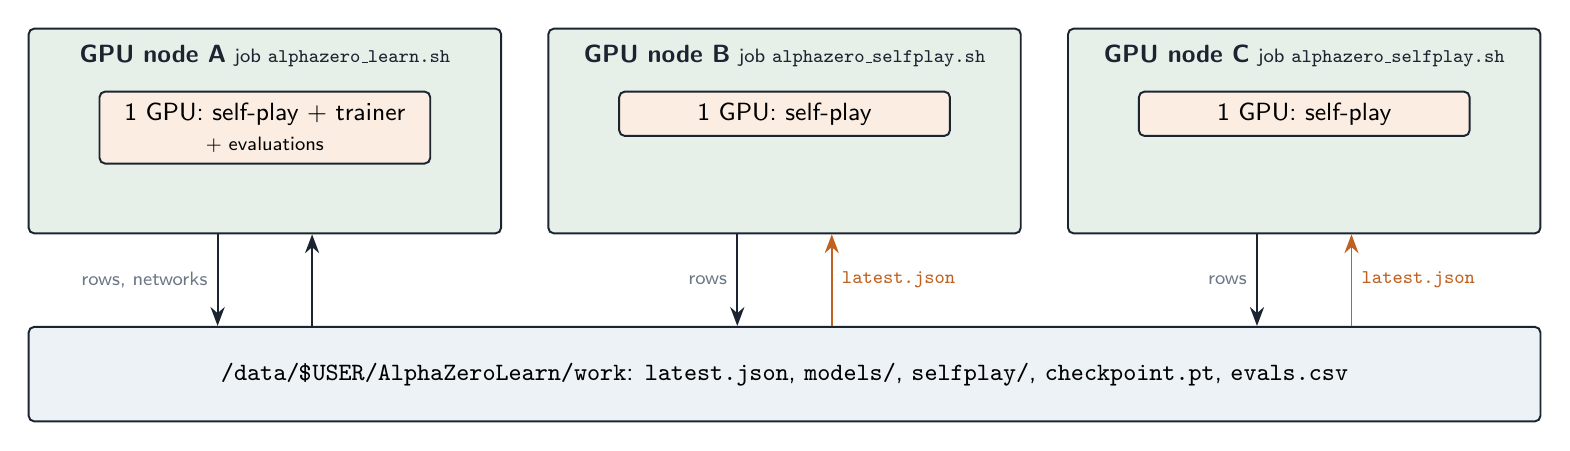
\begin{tikzpicture}[x=1mm,y=1mm]
  \node[boxb,minimum width=60mm,minimum height=26mm,anchor=north] (n1) at (0,0) {};
  \node[plain,anchor=north] at (0,-1) {\textbf{GPU node A}\ \scriptsize job \texttt{alphazero\_learn.sh}};
  \node[boxa,minimum width=42mm,anchor=north] at (0,-8) {1 GPU: self-play + trainer\\\scriptsize + evaluations};
  \node[boxb,minimum width=60mm,minimum height=26mm,anchor=north] (n2) at (66,0) {};
  \node[plain,anchor=north] at (66,-1) {\textbf{GPU node B}\ \scriptsize job \texttt{alphazero\_selfplay.sh}};
  \node[boxa,minimum width=42mm,anchor=north] at (66,-8) {1 GPU: self-play};
  \node[boxb,minimum width=60mm,minimum height=26mm,anchor=north] (n3) at (132,0) {};
  \node[plain,anchor=north] at (132,-1) {\textbf{GPU node C}\ \scriptsize job \texttt{alphazero\_selfplay.sh}};
  \node[boxa,minimum width=42mm,anchor=north] at (132,-8) {1 GPU: self-play};
  \node[box,minimum width=192mm,minimum height=12mm] (data) at (66,-44) {\texttt{/data/\$USER/AlphaZeroLearn/work}: \texttt{latest.json}, \texttt{models/}, \texttt{selfplay/}, \texttt{checkpoint.pt}, \texttt{evals.csv}};
  \draw[ar] ([xshift=-6mm]n1.south) -- node[tiny,left]{rows, networks} ([xshift=-6mm]data.north -| n1.south);
  \draw[ar] ([xshift=6mm]data.north -| n1.south) -- ([xshift=6mm]n1.south);
  \foreach \n in {n2,n3} {
    \draw[ar] ([xshift=-6mm]\n.south) -- node[tiny,left]{rows} ([xshift=-6mm]data.north -| \n.south);
    \draw[ar,draw=accent2] ([xshift=6mm]data.north -| \n.south) -- node[tiny,right,text=accent2]{\texttt{latest.json}} ([xshift=6mm]\n.south);
  }
\end{tikzpicture}
\end{document}
